\documentclass[11pt,a4paper]{article}
\usepackage{fontspec}
\setmainfont{TeX Gyre Pagella}
\newfontfamily\headfont{Inter}[UprightFont=*-ExtraBold,BoldFont=*-ExtraBold,Extension=.otf,Path=/usr/share/fonts/opentype/inter/]
\usepackage[a4paper,margin=2.3cm]{geometry}
\usepackage{graphicx,booktabs,float,caption,array,xcolor,longtable}
\usepackage{xurl}
\usepackage[hidelinks]{hyperref}
\usepackage{titlesec}
\usepackage[round]{natbib}
\usepackage{setspace}
\newfontfamily\ns{FreeSerif}
\newfontfamily\cjk{Noto Serif CJK SC}
\setstretch{1.05}
\renewcommand{\topfraction}{0.9}
\renewcommand{\bottomfraction}{0.8}
\renewcommand{\textfraction}{0.1}
\renewcommand{\floatpagefraction}{0.75}
\setlength{\parindent}{0pt}
\setlength{\parskip}{0.55em}
\titleformat{\section}{\headfont\Large}{\thesection}{0.8em}{}
\titleformat{\subsection}{\headfont\large}{\thesubsection}{0.8em}{}
\captionsetup{font=small,labelfont=bf}
\urlstyle{same}
\hypersetup{pdftitle={The Renamed World},pdfauthor={Tristan Hotham}}

\begin{document}
\begin{center}
{\Large\bfseries The Renamed World\par}
\vspace{0.4em}
{\large Official renamings of places in Wikidata, by decade and by wave\par}
\vspace{1.2em}
{\large Tristan Hotham\par}
\vspace{0.3em}
{\small Independent researcher\\
ORCID: 0000-0003-4931-9349\\
DOI: https://doi.org/10.5281/zenodo.24075301\par}
\vspace{0.8em}
2026
\end{center}

\begin{quote}
\small
\begin{center}\textbf{Abstract}\end{center}
Places change their official names in waves: revolutions and their undoing, wars and new borders, independence, nation-building and language policy, and the administrative reforms that merge villages into towns. I read every official name (Wikidata property P1448) that carries a start or end date on an item with coordinates, 79,554 names on 32,309 items, and reconstruct 17,025 dated changes of name on settlements and administrative areas. 47.9\% of these keep the name: new spellings (1,237), new status words (3,185) or a qualifier added or dropped (3,730). After removing a bulk revision of the Galician gazetteer and 170 duplicated records, 6,842 true renamings of 5,769 places in 78 present-day countries remain. Classified by explicit rules, 41.7\% came under revolution and communism, 7.7\% undid revolutionary or communist names, 13.0\% belong to nation-building and language policy, 8.0\% to mergers and administrative reform, 1.6\% to war and new borders and 0.3\% to decolonisation, a figure that reflects how few African and Asian renamings Wikidata dates, not the size of that wave; 27.7\% fit none of the rules. The busiest decade is the 1960s, driven by 596 Romanian village renamings in 1964; Ukraine's decommunisation of 2016 (261) and its renamings of 2024 (219) dominate the recent record. 303 places returned to an earlier name. Coverage is very uneven: 47.4\% of renamings are in the former Soviet Union and only 35 in Africa, so the counts describe Wikidata's record rather than the world.

\textbf{Keywords:} toponymy; place names; renaming; Wikidata; decommunisation; decolonisation; historical geography; critical place-name studies
\end{quote}

\section{Introduction}
Renaming a place is one of the cheapest and most visible things a new regime can do. Studies of the politics of place names have shown how street and town names commemorate, how they are changed when power changes hands, and how renaming writes a version of history into the everyday landscape \citep{azaryahu1996,roseredwood2010,light2004}. Most such work studies one city or one country in depth. This paper asks a simpler and broader question of an open, global source: when Wikidata records that a place's official name changed, when did that happen, where, and to which wave of renaming does it belong?

Wikidata \citep{wikidata} records the official name of many places with qualifiers for the date each name started and ended. That makes it possible to rebuild name histories in bulk, but also invites errors: a name that ends because a municipality was merged away is not a renaming, a new spelling is not a new name, and the same change is often recorded on two items. Much of the work reported here is about separating true renamings from these.

\section{Data}
The extract, made with the QLever SPARQL engine \citep{qlever}, holds every Wikidata item with coordinates (P625) and at least one official name (P1448) with a start time (P580) or end time (P582) qualifier: 118,507 rows, one per name statement and per class and country of the item, which reduce to 79,554 distinct names in 32,309 items. Names carry a language tag. Class (P31) and country (P17) are given only as identifiers. I grouped the commonest classes by hand from a sample of the labels of their items into settlements, administrative areas, streets and squares, stations, institutions and natural features, and the rest from words in each item's English label. The present-day country and continent of each item come from the Natural Earth 1:10m boundaries \citep{naturalearth}, with points within 30 km of a coast assigned to the nearest country; points in Crimea are counted with Ukraine. The analysis concerns the 17,025 name changes on settlements and administrative areas; the other kinds of thing (13,573 renamings of streets, stations, institutions and natural features) are released but not analysed.

\section{Method}
\subsection{From names to renamings}
Within each language of an item, a \emph{transition} is a name whose end date falls within one year of the start date of a different name. Transitions of one item in several languages within a year of each other form one \emph{event}, dated by the commonest start year. The old and new names shown are those in English where there is an English transition, otherwise in a local language of the present-day country. Names that end with no successor in any language are not events: 4,946 places have such names, mostly municipalities merged into a neighbour.

Each event is then compared, in the local languages where possible, after removing words for status (town, city, village, district, rural council, raion, county, prefecture, Bezirksamt, kota besar and the like, and the Chinese and Japanese suffixes for county, town, village and city) and the commonest Slavonic adjective endings. An event is a \emph{spelling} change if the names agree once accents, spacing and punctuation are ignored, if their similarity ratio is at least 0.8 and their lengths differ by three letters or fewer, or if their consonants agree; a \emph{status} change if the names agree once status words are removed; and a \emph{qualifier} change if the words of one name are a proper subset of the other's (Conflans to Conflans-sur-Anille). A name extended with an explicit conjunction (Lynton to Lynton and Lynmouth, Mirabel to Mirabel-et-Blacons) is a renaming, counted with mergers. None of the other flagged changes is counted as a renaming.

\subsection{Waves}
The remaining events are assigned to one wave by the first rule that applies (Table~\ref{tab:rules}). The communist vocabulary is a list of about 180 name parts in Latin, Cyrillic, Armenian and Georgian script: the names of Soviet and other communist leaders (Lenin, Stalin, Kirov, Kalinin, Zhdanov, Voroshilov, Frunze, Ordzhonikidze, Dimitrov, Gottwald and others), and words such as October, Soviet, Red Army, Komsomol, commune and May Day. Cyrillic is normalised so that Ukrainian and Russian spellings match.

\begin{table}[tbp]\centering\small\caption{Rules for the waves, applied in order; the first that applies decides. Full lists in code/rules.py.}\label{tab:rules}\begin{tabular}{rlp{10.2cm}}\toprule & Wave & Rule\\\midrule
1 & Undoing & Communist name part in the old name and not in the new, in a country under communist rule at some time, 1953 on; every Ukrainian renaming of 2015 to 2017 (made under the decommunisation laws); and the French restorations of 1800 to 1815 of names given in the 1790s\\
2 & Revolution and communism & Communist name part in the new name during communist rule, or a French renaming of 1790 to 1799\\
3 & War and new borders & Poland 1918 to 1922 and 1945 to 1950; Czechia 1945 to 1950; Kaliningrad, Karelia and Sakhalin after 1940 or 1945; Klaipeda, Istria, Slovenia, South Tyrol, Alsace-Moselle, Romania 1918 to 1925, North Schleswig\\
4 & Revolution and communism & Any other renaming under communist rule (USSR 1917 to 1989, eastern Europe 1945 to 1988, China, Vietnam and others to 1980), with communist rule starting only in 1939 in western Ukraine and western Belarus, 1940 in Chernivtsi, southern Bessarabia and Karelia, and 1945 in Transcarpathia, Kaliningrad and southern Sakhalin; sovkhoz settlements given names\\
5 & Mergers and reform & Settlements and areas in municipal merger programmes (Japan 1888 to 1890, 1953 to 1961, 1999 to 2010; France 1971 to 1977, 2015 on; Belgium, Denmark, Sweden, Germany, the Netherlands, Quebec, Greece); administrative reforms (Ukraine 2018 to 2020, Russia 2004 to 2006, Georgia 2006); names joined with and, et, und\\
6 & Decolonisation & From three years before to 25 years after independence, in former colonies in Africa, Asia, Oceania and the Caribbean\\
7 & Nation-building & Ireland from 1916, India and South Asia after independence, the former Soviet republics after 1991, eastern Europe after 1989, Turkey, Greece, Israel, Finland, Norway, the Baltic states, Spanish regions with their own languages from 1975, South Africa from 1994; later renamings in former colonies\\
8 & Mergers and reform & Any other renaming of an administrative area\\
9 & Other & Everything else\\
\bottomrule\end{tabular}\end{table}

\subsection{Checking}
I read every event in the three smallest waves (decolonisation, war and the undoing of names), every place renamed three times or more, every place named in this paper, and samples of 25 to 30 from each other wave and flag, repeating after each correction of the rules. The review changed the rules in ways listed in the repository notes; for example, Ukrainian rural councils were at first taken for spelling changes because their status words dominate the comparison, and settlement names of the form ``settlement of state farm No.~4'' were at first counted as communist names being undone. Three kinds of record were removed: a bulk revision of 1,859 Galician place names all dated 2026 (articles and spellings added to the regional gazetteer at once); 25 changes recorded twice on the same item with no change back in between; and 145 changes recorded on a second item for the same place within 5 km (a Romanian commune and its main village, a city and its district), keeping the settlement and then the item with the lower number. Two further events were excluded by hand (Table~\ref{tab:override}). In all 11.9\% of the name changes on places were removed as errors, duplicates or the Galician batch.

\section{Results}
\subsection{How many renamings}
Of 17,025 dated changes of name on places, 1,237 are new spellings, 3,185 new status words and 3,730 qualifiers added or dropped, leaving 6,842 renamings (40.2\%) of 5,769 places (Figure~\ref{fig:funnel}). Status changes are dominated by Japan, where 2,456 of 3,223 name changes are villages becoming towns or towns becoming cities.

\begin{figure}[tbp]\centering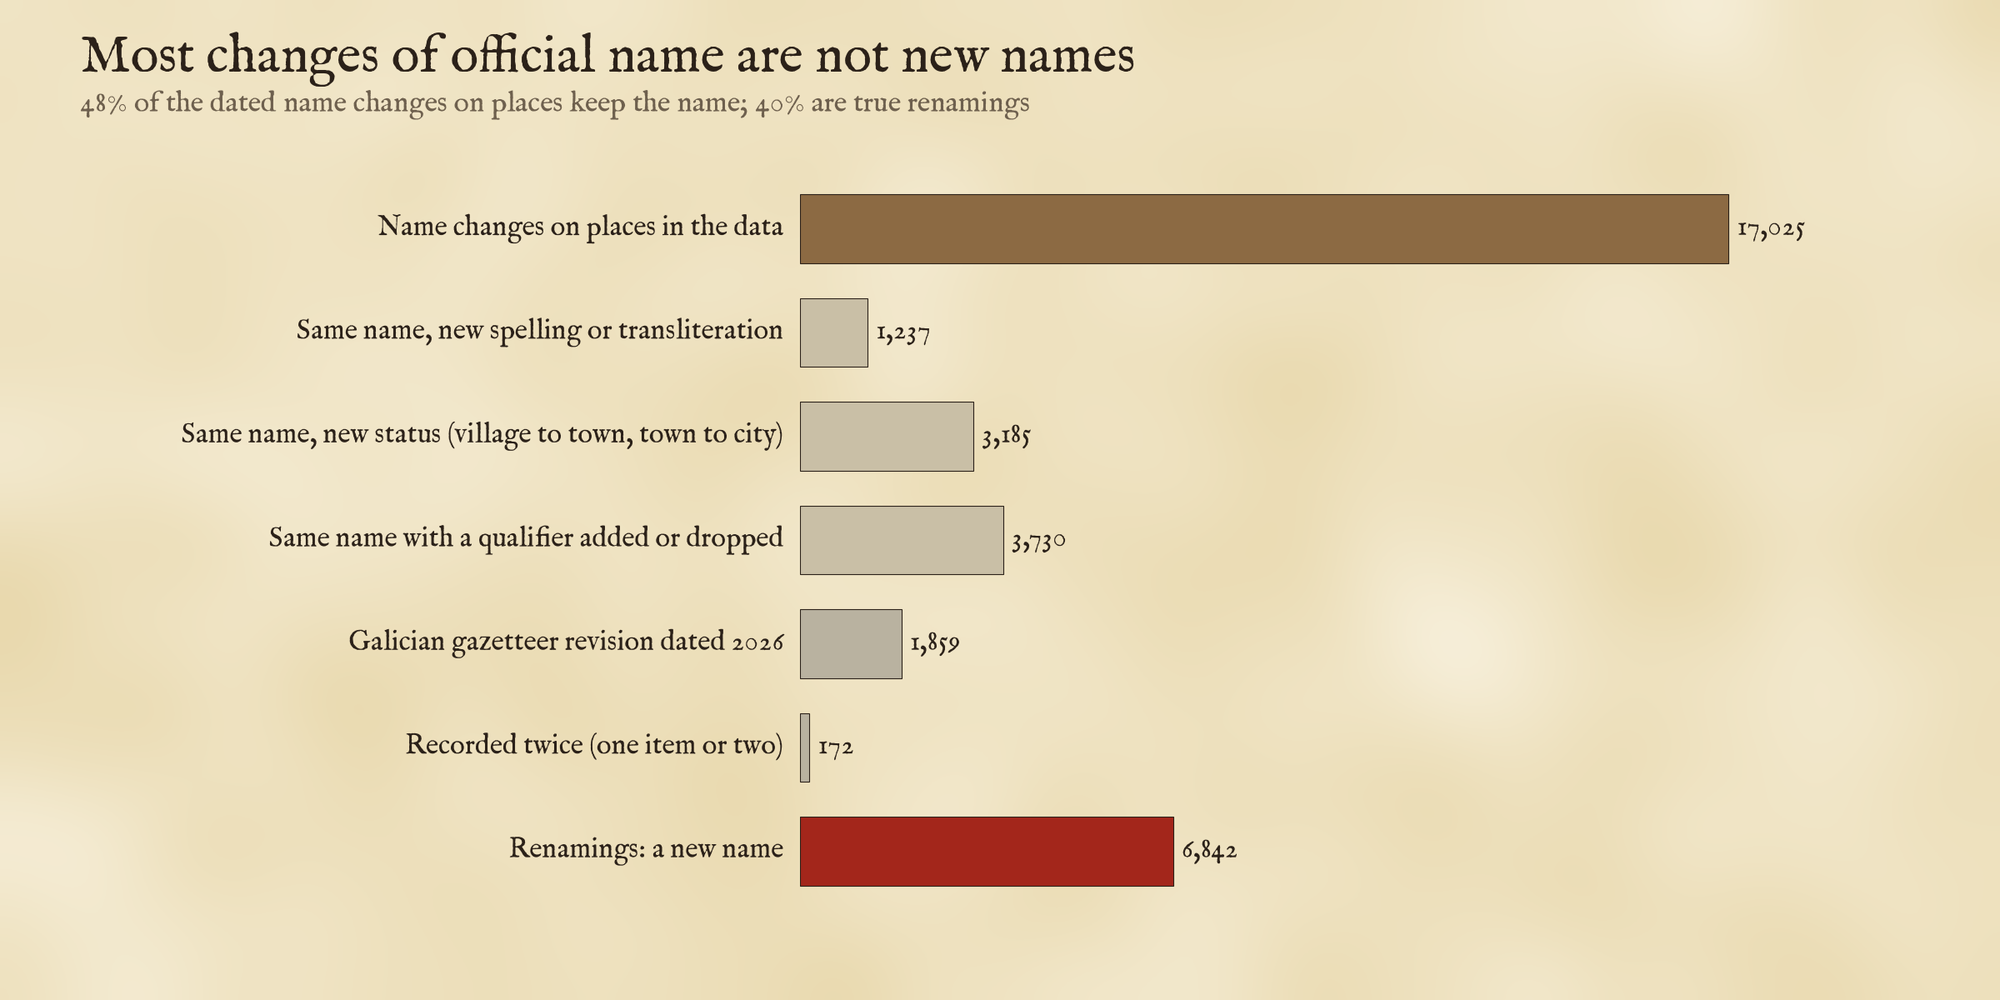
\includegraphics[width=0.92\textwidth]{f_funnel.png}
\caption{From dated changes of official name on places to renamings.}\label{fig:funnel}\end{figure}

\subsection{The waves and the decades}
Table~\ref{tab:waves} gives the size of each wave. Renamings under revolution and communism are the largest group (2,852): 337 gave a name that honours a communist leader, symbol or date, and most of the rest are village renamings ordered under communist rule, above all in Romania in 1964 and in Soviet Ukraine and Armenia. 529 renamings undid such names: 16 during de-Stalinisation, 114 after the fall of communism, and 360 under Ukraine's decommunisation laws from 2015 (every Ukrainian renaming of 2015 to 2017 is counted here, since the renamings of those years were made under those laws). Nation-building and language policy (890) is mostly the former Soviet republics after 1991, from Kazakh and Azerbaijani names replacing Russian ones to Ukraine's renamings of 2024 under a 2023 law against names tied to Russia (219, of which 91 removed surviving Soviet names and so count as undoing).

\begin{table}[tbp]\centering\small\caption{Renamings of places by wave: number, share, number of present-day countries, busiest decade and the three countries (ISO codes) with most.}\label{tab:waves}\begin{tabular}{lrrrrl}\toprule Wave & n & \% & Countries & Peak & Most in\\\midrule
Decolonisation & 22 & 0.3 & 12 & 1960s & CD, DZ, ZM\\
Revolution and communism & 2,852 & 41.7 & 28 & 1960s & RO, UA, RU\\
Undoing revolutionary and communist names & 529 & 7.7 & 15 & 2010s & UA, RU, KZ\\
War and new borders & 107 & 1.6 & 5 & 1940s & RU, RO, PL\\
Nation-building and language policy & 890 & 13.0 & 38 & 1990s & UA, ID, AZ\\
Mergers and administrative reform & 548 & 8.0 & 27 & 2010s & CN, JP, FR\\
Other renamings & 1,894 & 27.7 & 54 & 1930s & FR, JP, CA\\
\midrule All renamings & 6,842 & 100.0 & 78 & 1960s & \\
\bottomrule\end{tabular}\end{table}

Figure~\ref{fig:decades} shows the renamings by decade. Before 1900 almost all are local (other). The 1920s to 1940s are communist, with the war years adding the German names of the territories that became Polish and Russian in 1945. The busiest decade is the 1960s (1,242), and the busiest single year is 1964 in Romania (596). After 1990 nation-building and the undoing of communist names take over; 2016 in Ukraine (261) is the second busiest year in the record.

\begin{figure}[tbp]\centering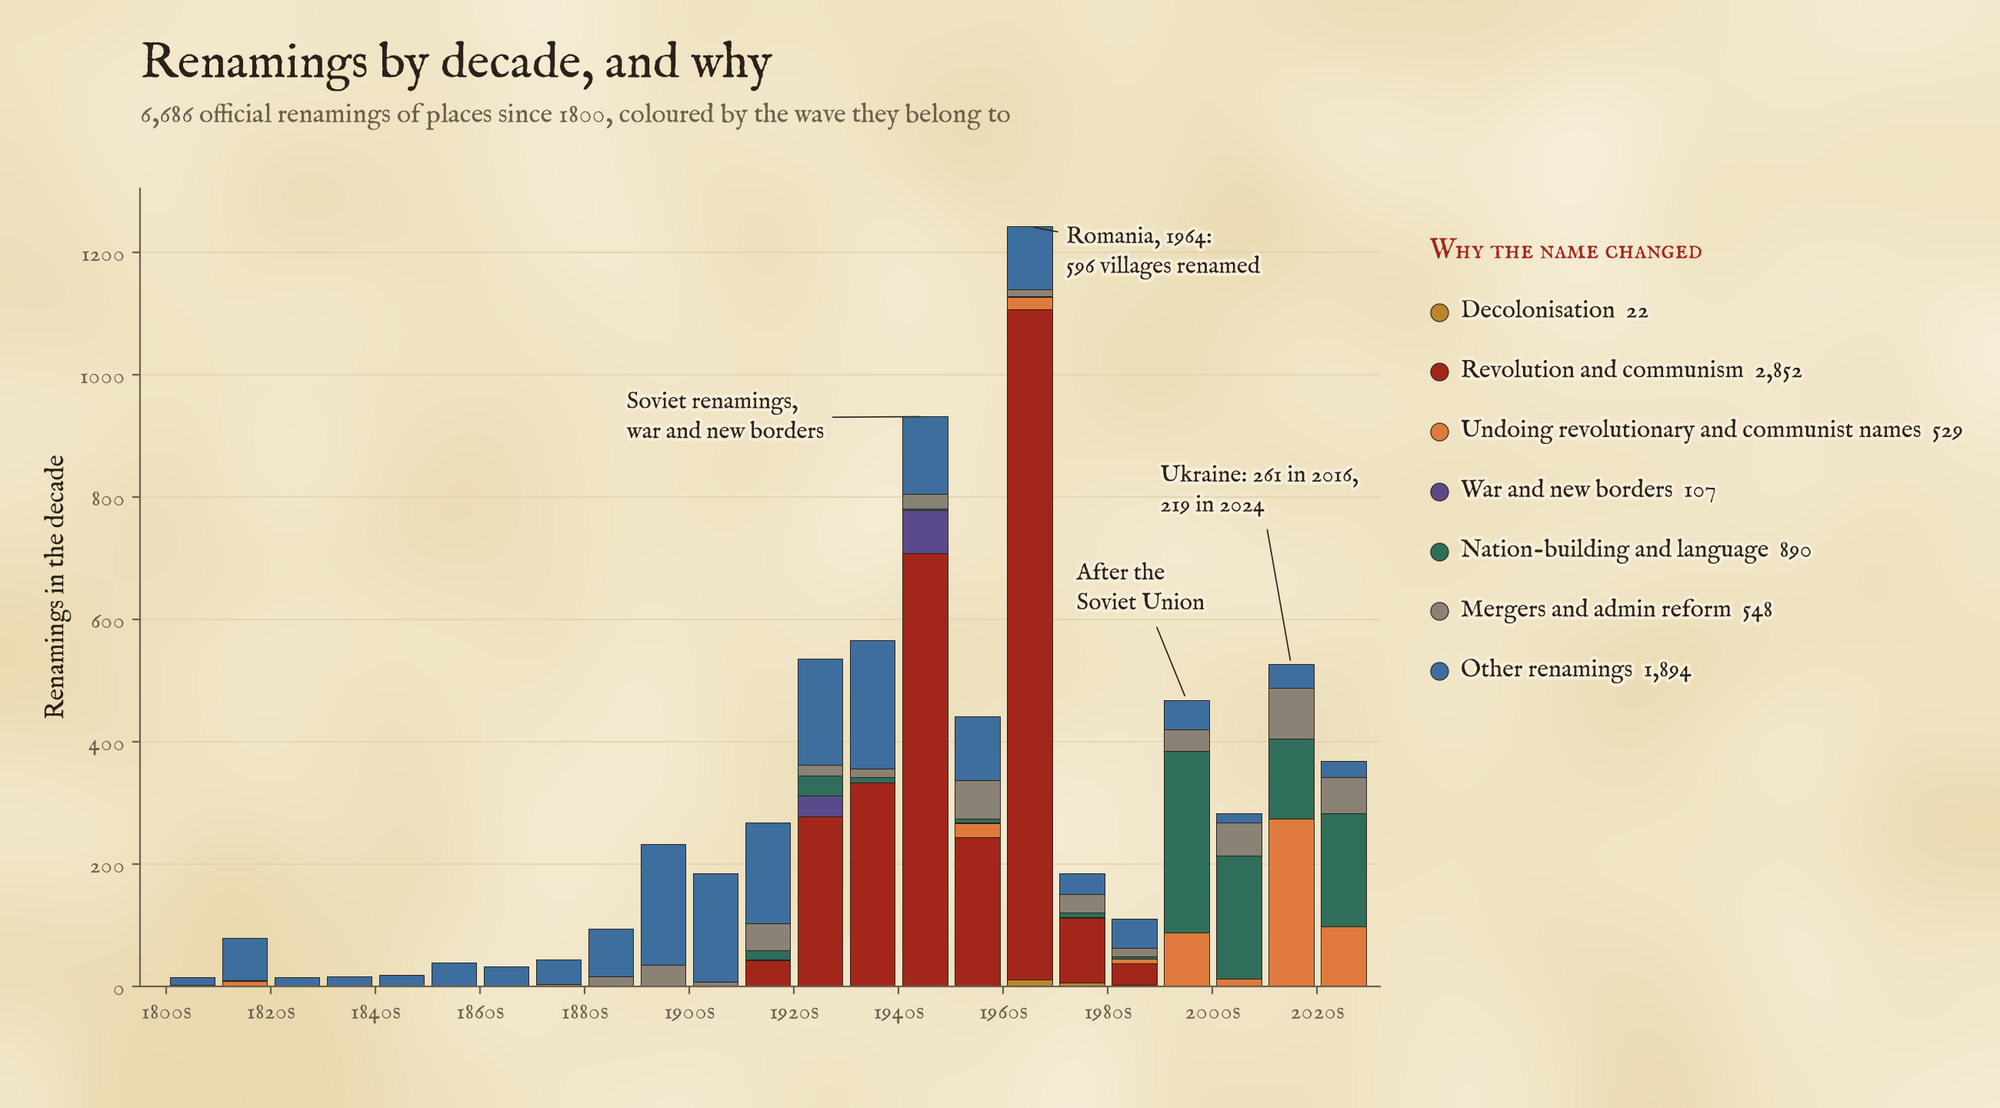
\includegraphics[width=\textwidth]{f_decades.png}
\caption{Renamings of places by decade since 1800, by wave.}\label{fig:decades}\end{figure}

\subsection{Where}
The record leans heavily east (Figures~\ref{fig:map} and \ref{fig:europe}, Table~\ref{tab:countries}). 3,245 renamings (47.4\%) are in the former Soviet Union, and the five countries with most hold 64.9\%. Decolonisation, which in the literature and in popular memory is one of the great waves of renaming, appears only 22 times, 7 of them in the Democratic Republic of the Congo (Léopoldville to Kinshasa, Élisabethville to Lubumbashi). This is an artefact of the record and of the rule, not a finding. Of twenty well-known renamings away from colonial names in Africa and Asia, 7 (among them Calcutta to Kolkata, Dacca to Dhaka, Bathurst to Banjul and Tananarive to Antananarivo) have no dated official name in the extract at all; 2 (Batavia to Jakarta, Usumbura to Bujumbura) have official names but no dated change; 4 fall in other waves, Bombay to Mumbai, Madras to Chennai and Rangoon to Yangon as nation-building because they came more than 25 years after independence, and Saigon to Ho Chi Minh City as communist; and only 7 are counted as decolonisation. Africa as a whole has 35 renamings, India 4. The United Kingdom has 23, nearly all civil parishes and urban districts taking a joined name, and Ireland none: the returns of Kingstown to Dún Laoghaire and Queenstown to Cobh are not recorded with dates.

\begin{figure}[tbp]\centering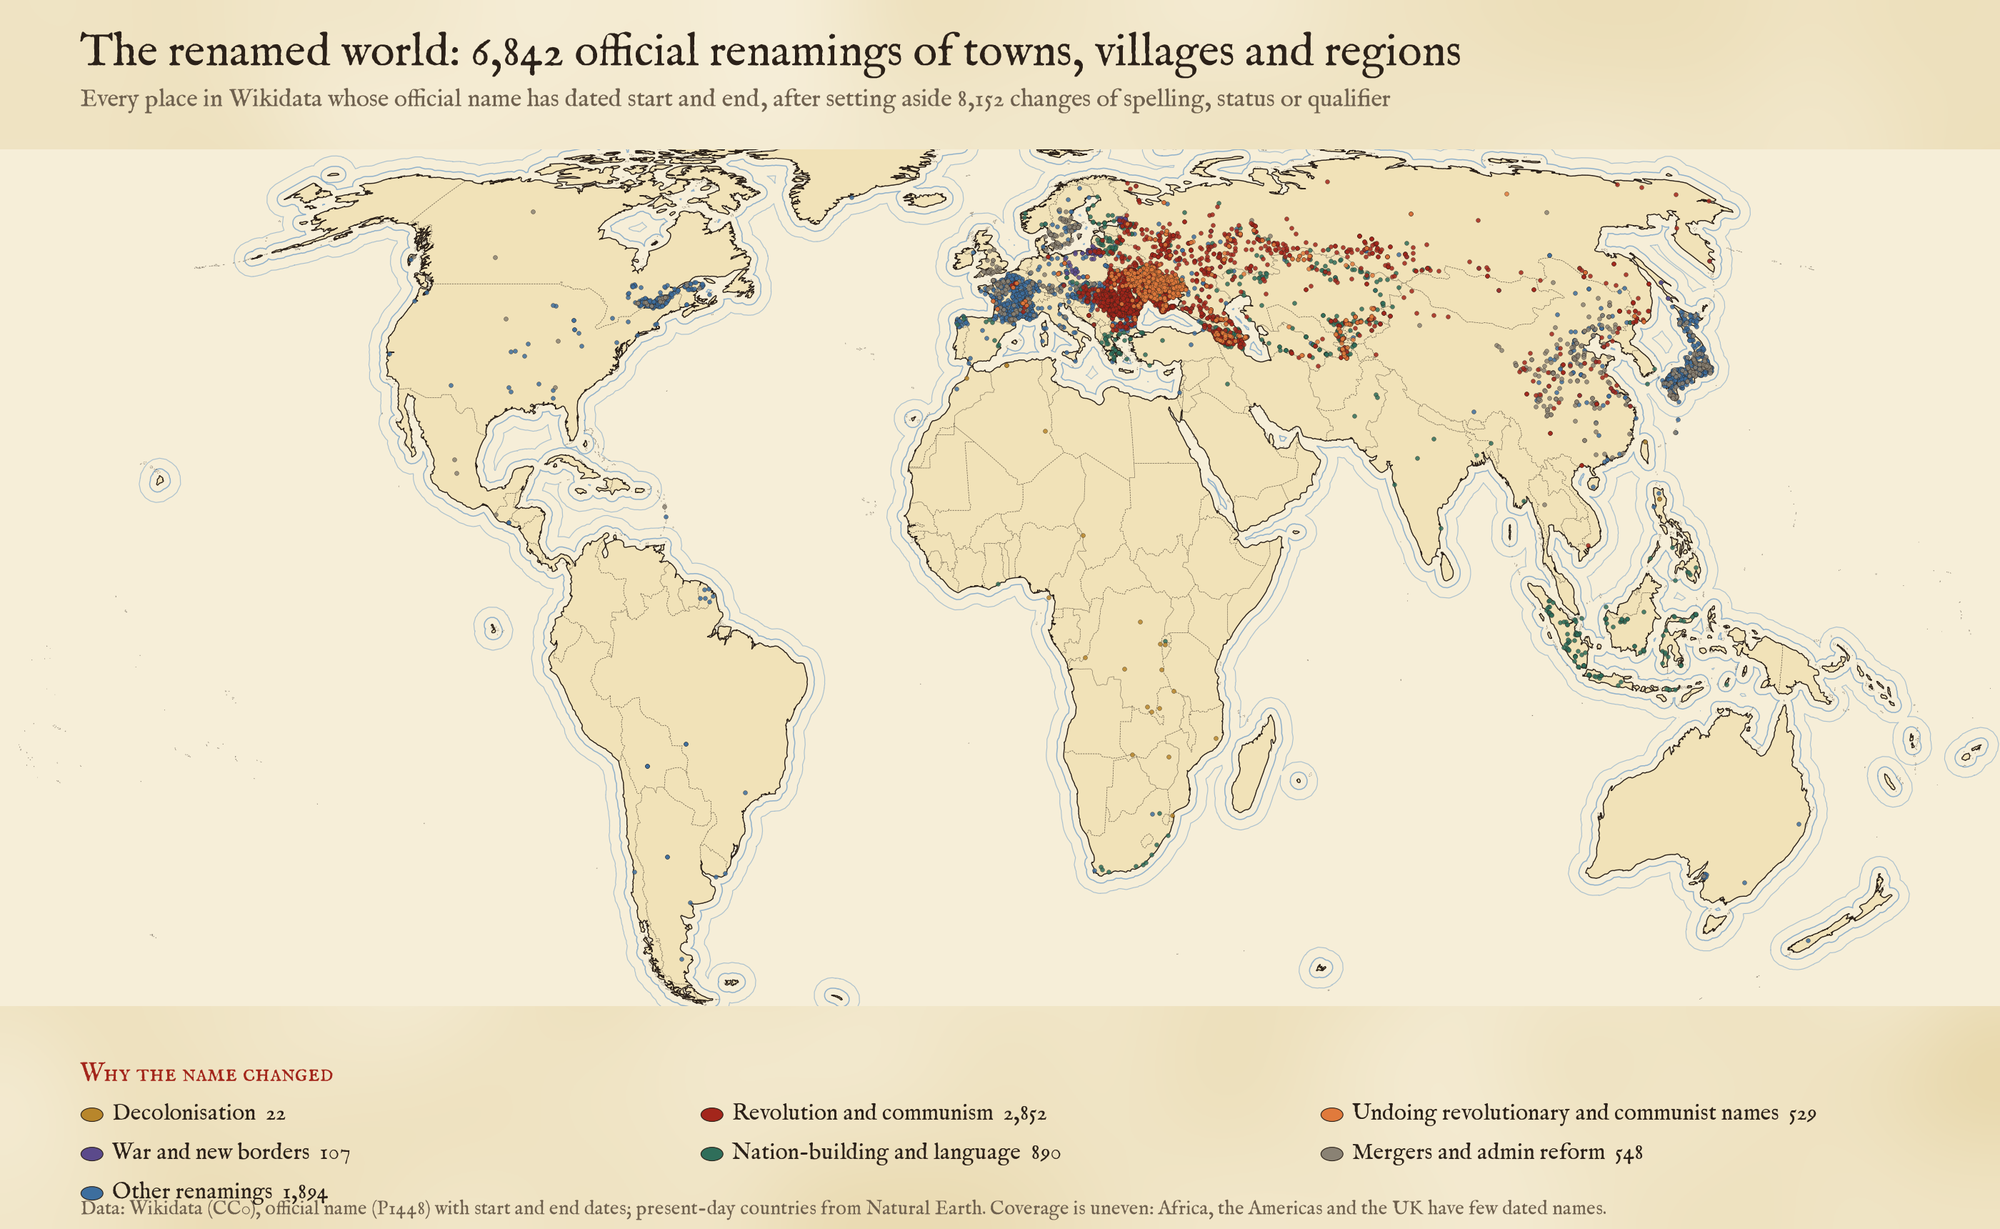
\includegraphics[width=\textwidth]{f_map.png}
\caption{Every renaming of a place, coloured by wave (equal-earth projection).}\label{fig:map}\end{figure}

\begin{figure}[tbp]\centering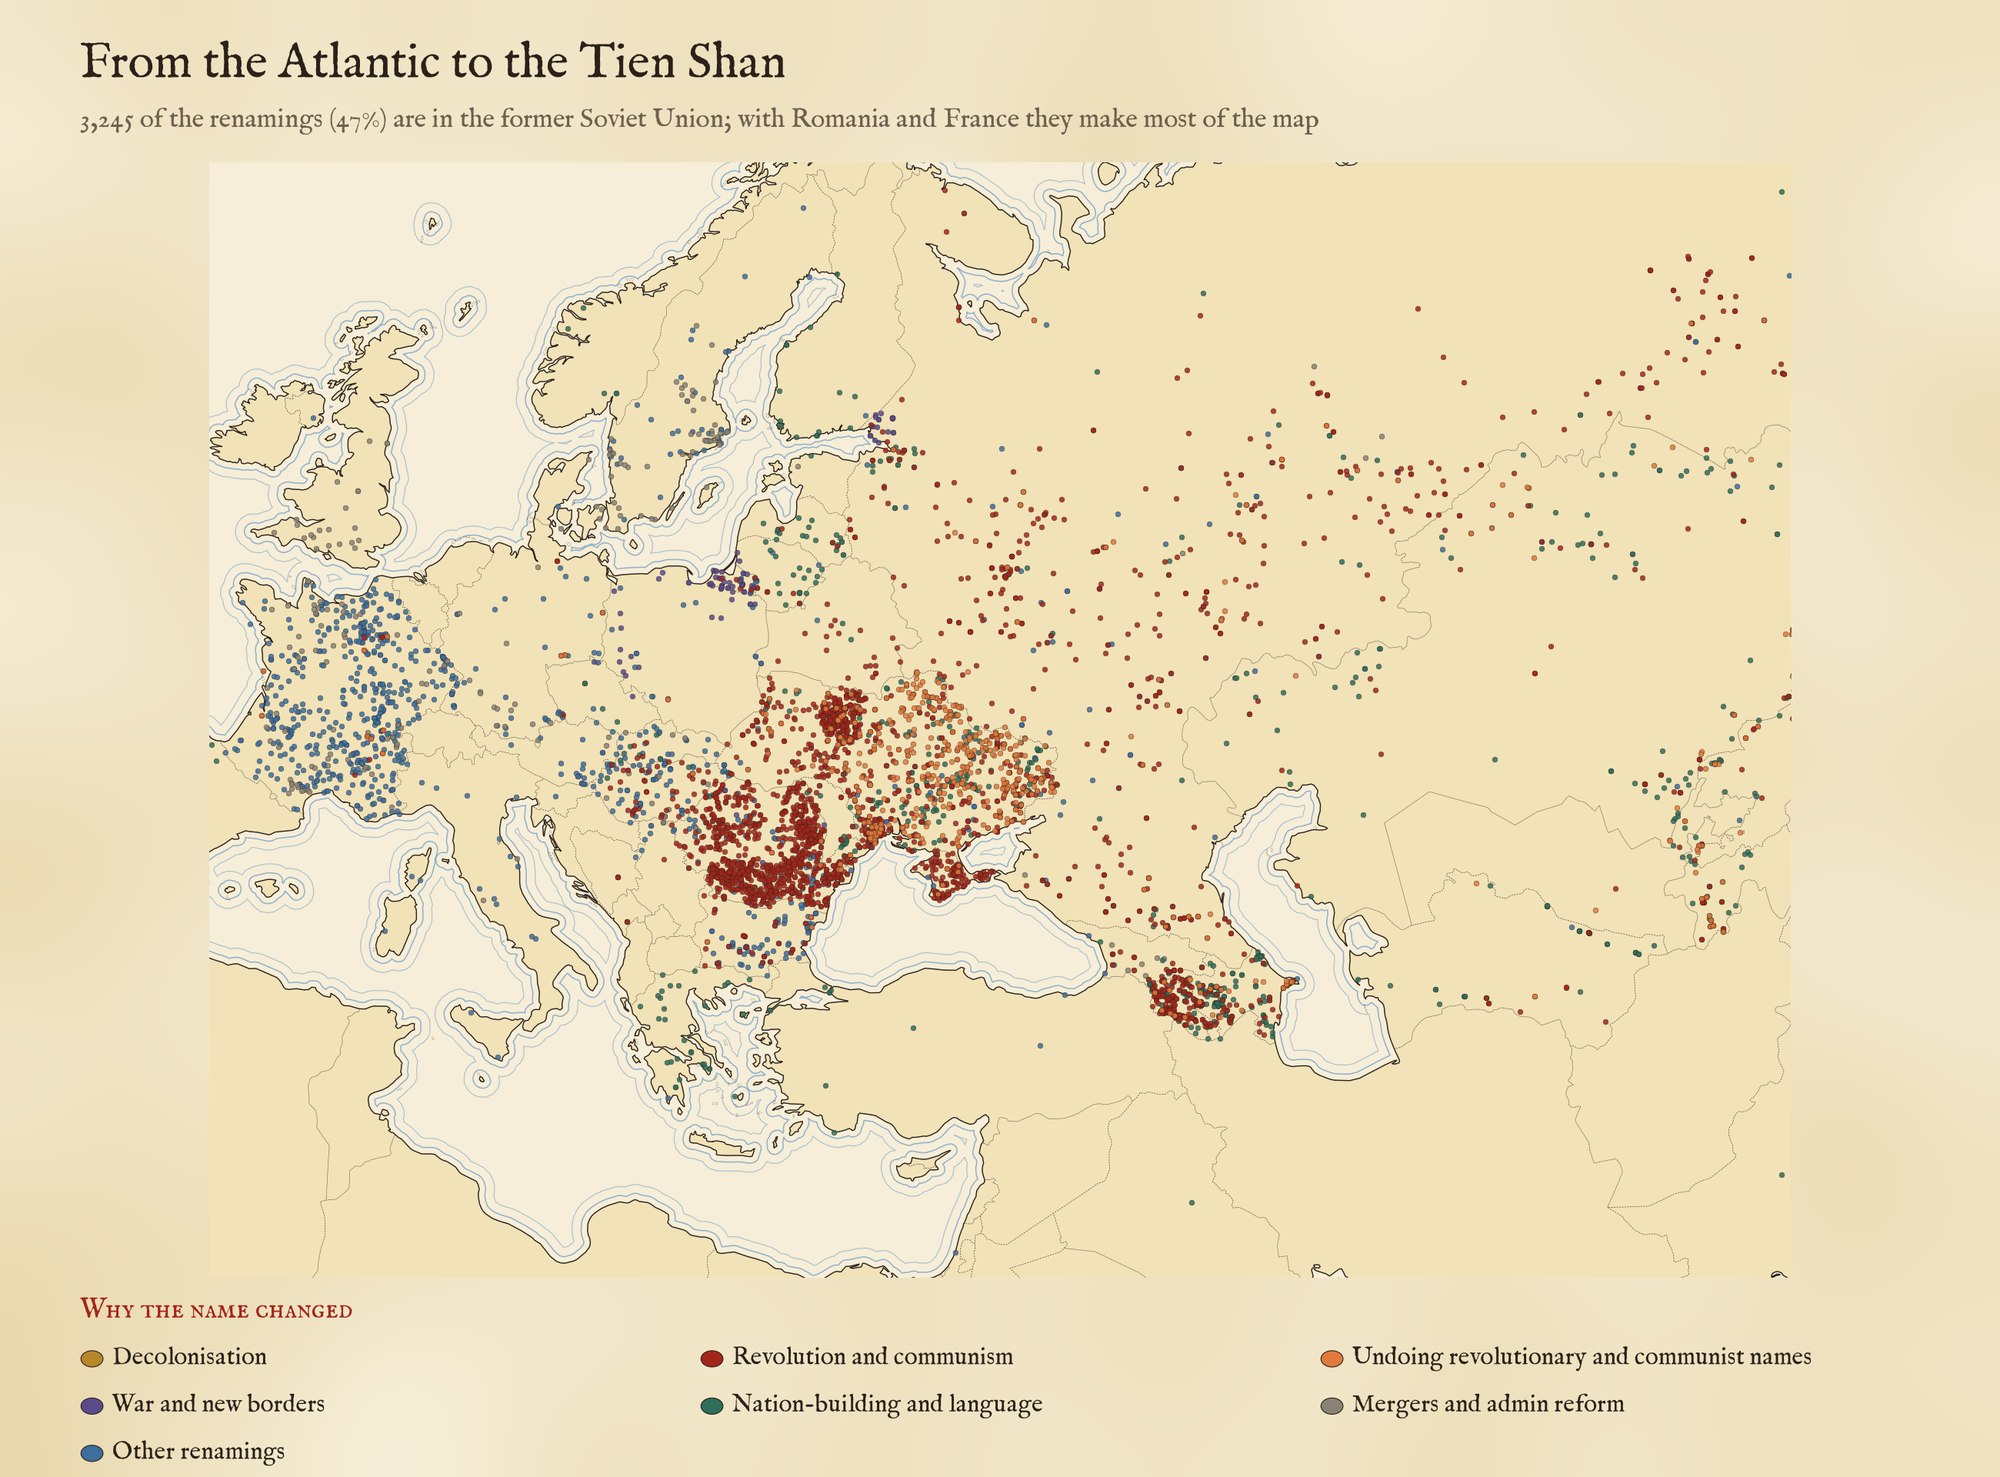
\includegraphics[width=\textwidth]{f_europe.png}
\caption{Renamings from the Atlantic to Central Asia.}\label{fig:europe}\end{figure}

\begin{table}[tbp]\centering\footnotesize\caption{The fifteen countries with most renamings, by wave: decolonisation (Dec), revolution and communism (Com), undoing (Und), war (War), nation-building (Nat), mergers and reform (Mer), other (Oth).}\label{tab:countries}\begin{tabular}{lrrrrrrrrr}\toprule Country & n & Places & Dec & Com & Und & War & Nat & Mer & Oth\\\midrule
Ukraine & 1,515 & 1,190 & 0 & 867 & 386 & 0 & 174 & 3 & 85\\
Romania & 1,053 & 944 & 0 & 876 & 5 & 36 & 33 & 2 & 101\\
Russia & 777 & 591 & 0 & 513 & 46 & 46 & 55 & 14 & 103\\
France & 563 & 524 & 0 & 13 & 8 & 0 & 0 & 71 & 471\\
Japan & 532 & 519 & 0 & 0 & 0 & 0 & 0 & 119 & 413\\
China & 314 & 246 & 0 & 62 & 0 & 0 & 0 & 171 & 81\\
Armenia & 290 & 222 & 0 & 214 & 8 & 0 & 62 & 0 & 6\\
Canada & 221 & 206 & 0 & 0 & 0 & 0 & 0 & 26 & 195\\
Azerbaijan & 184 & 150 & 0 & 52 & 20 & 0 & 105 & 2 & 5\\
Kazakhstan & 183 & 145 & 0 & 49 & 23 & 0 & 100 & 0 & 11\\
Indonesia & 126 & 126 & 0 & 0 & 0 & 0 & 126 & 0 & 0\\
Bulgaria & 115 & 83 & 0 & 31 & 3 & 0 & 0 & 0 & 81\\
Hungary & 113 & 98 & 0 & 39 & 1 & 0 & 4 & 8 & 61\\
Sweden & 88 & 86 & 0 & 0 & 0 & 0 & 0 & 53 & 35\\
Germany & 75 & 63 & 0 & 5 & 3 & 0 & 0 & 17 & 50\\
\bottomrule\end{tabular}\end{table}

\subsection{Name histories}
860 places were renamed twice or more and 158 three times or more (Figure~\ref{fig:chains}, Table~\ref{tab:most}). The capital of Kazakhstan was renamed 6 times, as often as any place in the record: Ak-Mola, Akmolinsk, Tselinograd, Akmola, Astana, Nur-Sultan and Astana again. Vladikavkaz went from Ordzhonikidze to Dzaudzhikau and back to Ordzhonikidze before regaining its name in 1990; Luhansk was Voroshilovgrad twice; Rybinsk was named after Shcherbakov in 1946 and Andropov in 1984. 338 renamings, of 303 places, returned to a name the place had held before, 89 of them undoing a revolutionary or communist name. The oldest in the record are French: names given in the Revolution of the 1790s, such as Commune-Affranchie for Lyon and Commune-Franklin for Bordeaux, which Wikidata records as reversed in 1814.

\begin{figure}[tbp]\centering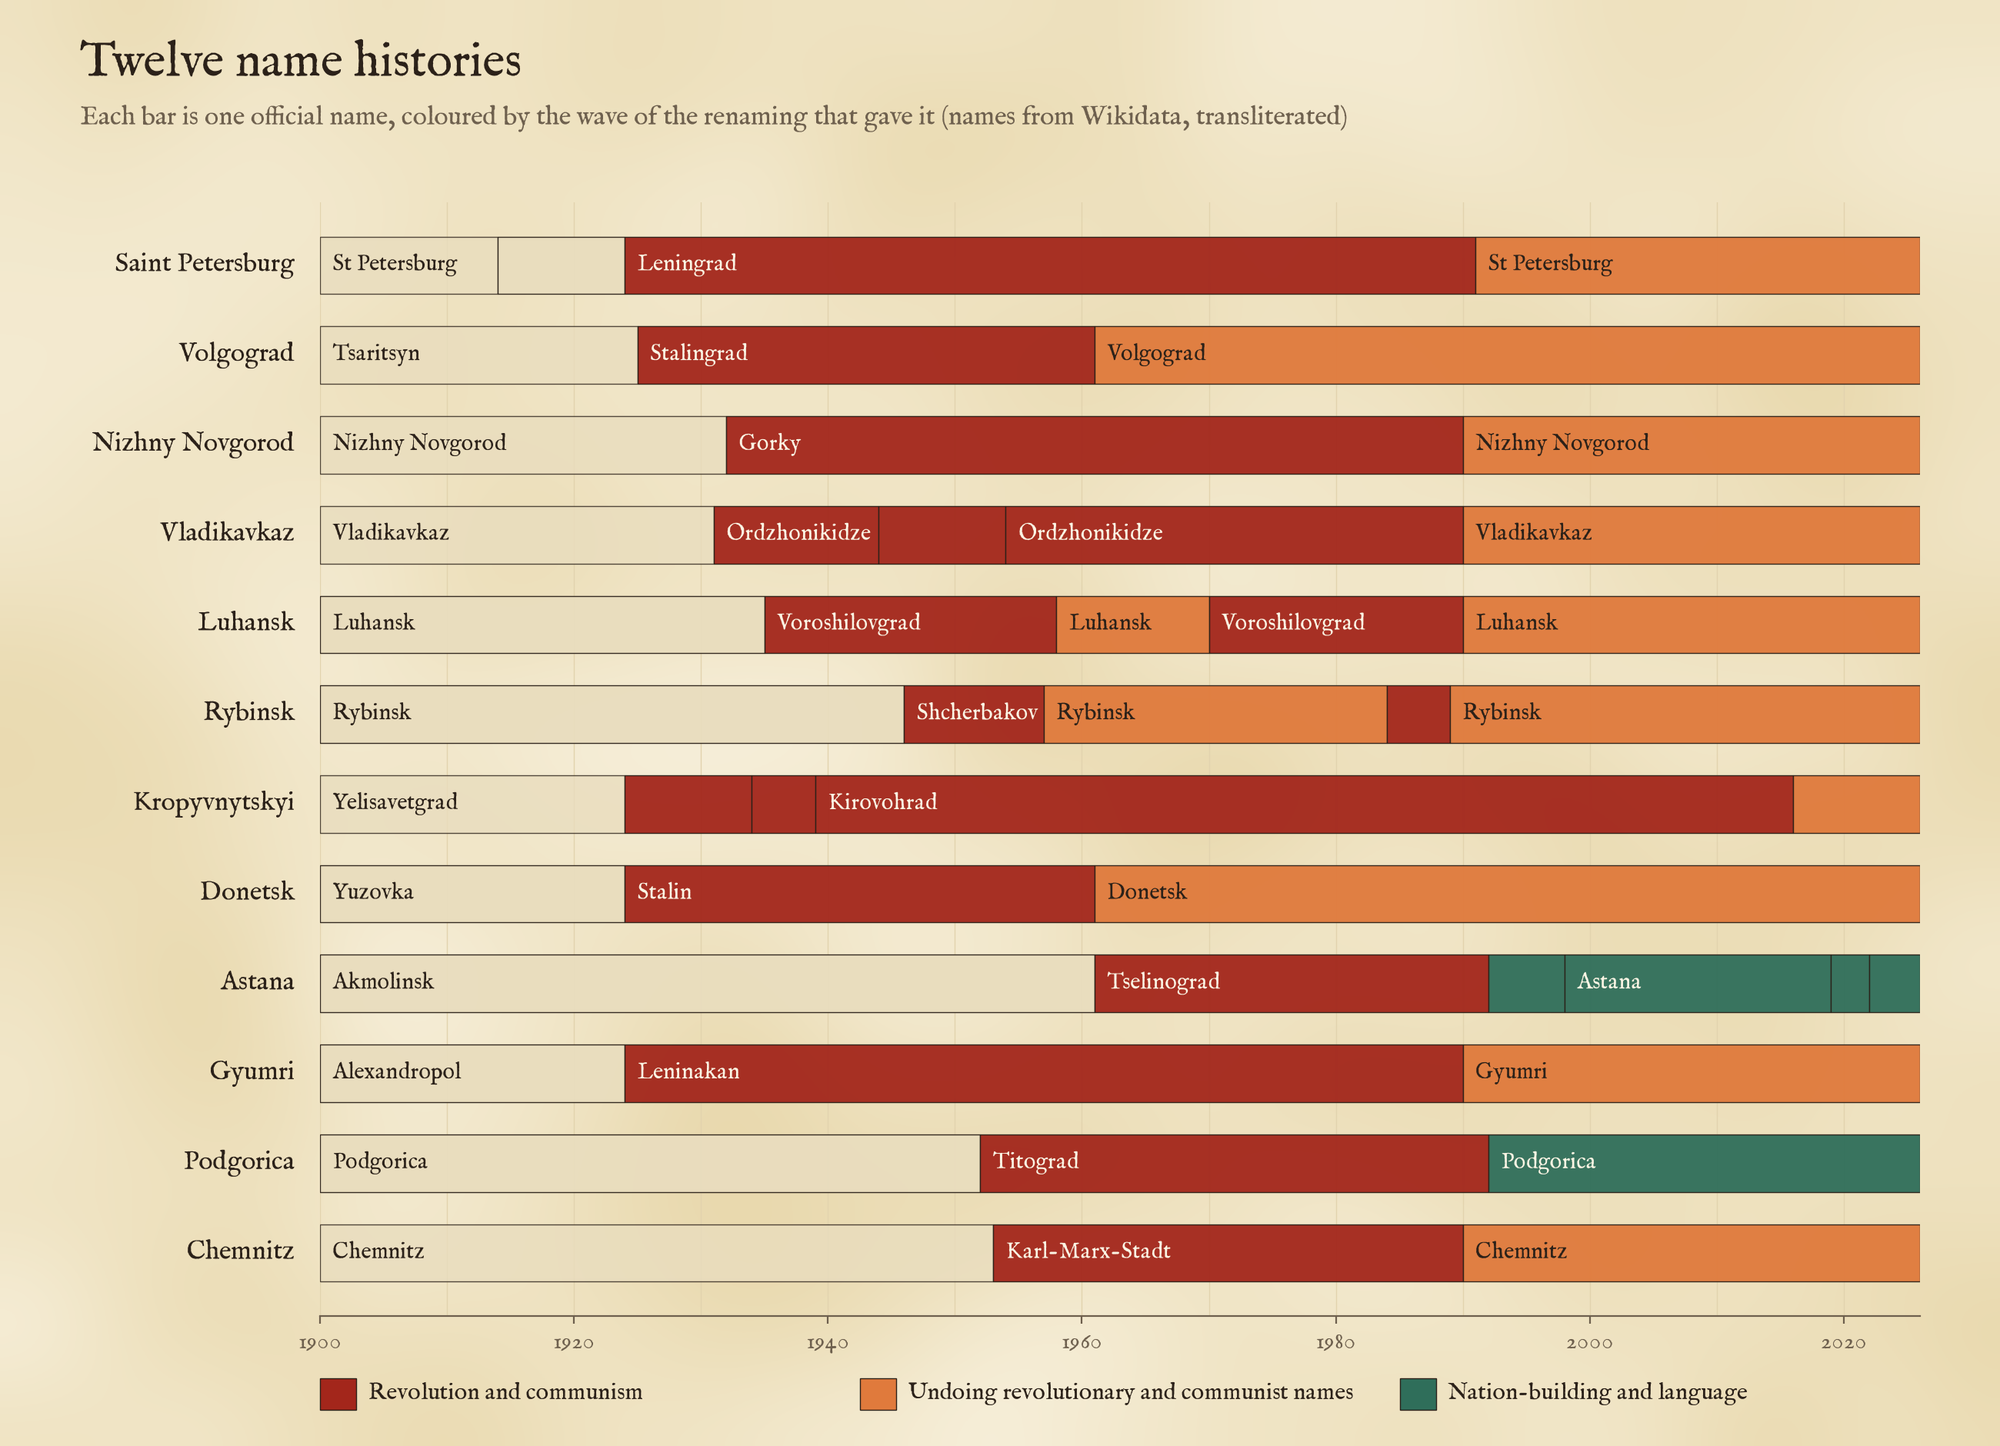
\includegraphics[width=\textwidth]{f_chains.png}
\caption{Name histories of twelve places since 1900. Each bar is one official name, coloured by the wave of the renaming that gave it. Names transliterated from the Wikidata records.}\label{fig:chains}\end{figure}

\begin{table}[tbp]\centering\small\caption{Events corrected by hand.}\label{tab:override}\begin{tabular}{lllp{10cm}}\toprule Item & Year & Action & Reason\\\midrule
Q103892 & 1920 & exclude & Zabrze: a German name with the Polish name in brackets during the Upper Silesian plebiscite years; not an official renaming\\
Q103892 & 1922 & exclude & Zabrze: the bracketed form dropped again; not an official renaming\\
\bottomrule\end{tabular}\end{table}
{\footnotesize\begin{longtable}{p{2.6cm}lrp{7.6cm}p{2.4cm}}\caption{The places renamed most often (official names in the language of the renamings, as recorded in Wikidata).}\label{tab:most}\\\toprule Place & & n & Names & Years\\\midrule\endfirsthead
\multicolumn{5}{l}{\small Table \ref{tab:most}, continued}\\\toprule Place & & n & Names & Years\\\midrule\endhead
Astana & KZ & 6 & {\ns Ак-Мола > Акмолінськ > Целиноград > Акмола > Астана > Нур-Султан > Астана} & 1832, 1961, 1992, 1998, 2019, 2022\\
Rybinsk & RU & 6 & {\ns Усть-Шексна > Рыбная слобода > Рыбинск > Щербаков > Рыбинск > Андропов > Рыбинск} & 1504, 1777, 1946, 1957, 1984, 1989\\
Priozersk & RU & 6 & {\ns Корела > Кексгольм > Корела > Кексгольм > Кякисалми > Кексгольм > Приозерск} & 1580, 1595, 1611, 1917, 1940, 1948\\
Velykodolynske & UA & 5 & {\ns Грос-Лібенталь > Велика Аккаржа > Спартаковка > Большая Аккаржа > Грос-Лібенталь > Великодолинське} & 1918, 1933, 1939, 1941, 1945\\
Lustdorf & UA & 5 & {\ns Кайзерхайм > Люстер > Люстдорф > Ольгіно > Чорноморка > Люстдорф} & 1805, 1886, 1907, 1945, 1991\\
Luhansk & UA & 5 & {\ns Луганский завод > Луганск > Ворошиловград > Луганськ > Ворошиловград > Луганськ} & 1882, 1935, 1958, 1970, 1990\\
Dobrich & BG & 5 & {\ns Хаджиоглу Пазарджик > Добрич > Базаржик > Добрич > Толбухин > Добрич} & 1882, 1916, 1940, 1949, 1990\\
Oktyabrskoye & RU & 5 & {\ns Шолхи > Камбилеевская > Тарский > Шолхи > Карца > Октябрьское} & 1859, 1867, 1922, 1944, 1965\\
Saritsın & RU & 5 & {\ns Чёрногрязская > Чёрная Грязь > Богородское > Чёрная Грязь > Царицыно > Ленино} & 1633, 1684, 1712, 1775, 1918\\
Kadiivka & UA & 5 & {\ns Шубінка > Кадіївка > Серго > Кадіївка > Стаханов > Кадіївка} & 1898, 1937, 1943, 1978, 2016\\
Huangzhou District & CN & 5 & {\ns {\cjk 黄冈县} > {\cjk 黄州镇} > {\cjk 黄冈县} > {\cjk 黄州区} > {\cjk 黄冈县} > {\cjk 黄州市}} & 1951, 1955, 1983, 1987, 1990\\
Shenyang & CN & 4 & {\ns Мукден > Фэнтянь > Шэньян > Мукден > Шэньян} & 1912, 1929, 1932, 1945\\
Budyonnovsk & RU & 4 & {\ns Святой Крест > Прикумск > Будённовск > Прикумск > Будённовск} & 1921, 1935, 1957, 1973\\
Shlisselburg & RU & 4 & {\ns Орешек > Нотебург > Шлиссельбург > Петрокрепость > Шлиссельбург} & 1611, 1702, 1944, 1993\\
Kropyvnytskyi & UA & 4 & {\ns Єлисаветград > Зінов'євськ > Кірово > Кіровоград > Кропивницький} & 1924, 1934, 1939, 2016\\
Alchevsk & UA & 4 & {\ns Юр'ївка > Алчевське > Ворошиловськ > Комунарськ > Алчевськ} & 1903, 1926, 1961, 1991\\
Chystiakove & UA & 4 & {\ns Олексіївка > Олексієве-Леонове > Чистякове > Torez > Chystiakove} & 1840, 1868, 1964, 2016\\
Molchanovsky District & RU & 4 & {\ns Молчановский район > Кривошеинский район > Молчановский район > Кривошеинский район > Молчановский район} & 1930, 1939, 1963, 1965\\
Ghafurov & TJ & 4 & {\ns Стансияи-Ленинобод > Советобод > Хуҷанд > Советобод > Ғафуров} & 1953, 1962, 1964, 1978\\
La Roche-sur-Yon & FR & 4 & {\ns La Roche-sur-Yon > Napoléon > Bourbon-Vendée > Napoléon > La Roche-sur-Yon} & 1804, 1814, 1848, 1870\\
\bottomrule\end{longtable}}

\section{Limitations}
The counts describe Wikidata, not the world. Dated official names have been added in bulk for some countries (Ukraine, Romania, Russia, France, Japan) and hardly at all for others, so comparisons between countries and continents mostly measure editing effort. Dates are as recorded, which may be the date of a decree, of its publication or of its coming into force, and a few are plainly wrong (the French restorations dated 1814). The waves are assigned by rules from country, date and the words in names, not by reading the reason for each renaming; a renaming can have several motives, and the rules will misplace some, for example a Soviet-era renaming that was in fact local, or a post-1991 renaming that undid a communist name not on the vocabulary list. Countries are present-day ones, and the start of communist rule is moved later only for the regions listed in Table~\ref{tab:rules}; renamings made under German or Romanian occupation in 1941 to 1944 inside the Soviet Union are still counted with Soviet rule. The decolonisation wave is the clearest case of missing data (Section~4.3): its size says nothing about how many places were renamed at independence. The spelling test can join different names that happen to look alike, and the status words do not cover every language. Places that were merged and lost their name are not renamings here, though for the people who lived there they may have felt like one.

\section{Data availability}
The interactive map is at \url{https://maps.tristanhotham.com/renamed-world/}. Data and code are at \url{https://github.com/Tristan-Hotham/renamed-world}: \texttt{renamings.csv} lists every dated change of name on places with its flags, wave, the reason for any exclusion and the language of the names; \texttt{renamings\_other\_kinds.csv} the renamings of streets, stations, institutions and natural features; \texttt{overrides\_applied.csv} the hand corrections; and \texttt{results.json} every number in this paper. The rules are in \texttt{code/rules.py}. Wikidata content is CC0; derived data CC0; text and figures CC BY 4.0; code MIT.

\section*{AI assistance}
I wrote the text, with drafting and editing assistance from Claude (Anthropic), which also helped prepare the analysis code. I reviewed and checked all text and results.

\begin{thebibliography}{9}
\bibitem[Azaryahu(1996)]{azaryahu1996} Azaryahu, M. (1996) The power of commemorative street names. \textit{Environment and Planning D: Society and Space} 14(3), 311 to 330.
\bibitem[Bast and Buchhold(2017)]{qlever} Bast, H. and Buchhold, B. (2017) QLever: a query engine for efficient SPARQL+text search. \textit{Proceedings of the 2017 ACM Conference on Information and Knowledge Management (CIKM)}, 647 to 656.
\bibitem[Light(2004)]{light2004} Light, D. (2004) Street names in Bucharest, 1990 to 1997: exploring the modern historical geographies of post-socialist change. \textit{Journal of Historical Geography} 30(1), 154 to 172.
\bibitem[Natural Earth(2026)]{naturalearth} Natural Earth (2026) Admin 0 countries, 1:10m. Public domain. \url{https://www.naturalearthdata.com/}
\bibitem[Rose-Redwood et al.(2010)]{roseredwood2010} Rose-Redwood, R., Alderman, D. and Azaryahu, M. (2010) Geographies of toponymic inscription: new directions in critical place-name studies. \textit{Progress in Human Geography} 34(4), 453 to 470.
\bibitem[Vrande\v{c}i\'c and Kr\"otzsch(2014)]{wikidata} Vrande\v{c}i\'c, D. and Kr\"otzsch, M. (2014) Wikidata: a free collaborative knowledgebase. \textit{Communications of the ACM} 57(10), 78 to 85.
\end{thebibliography}
\end{document}
